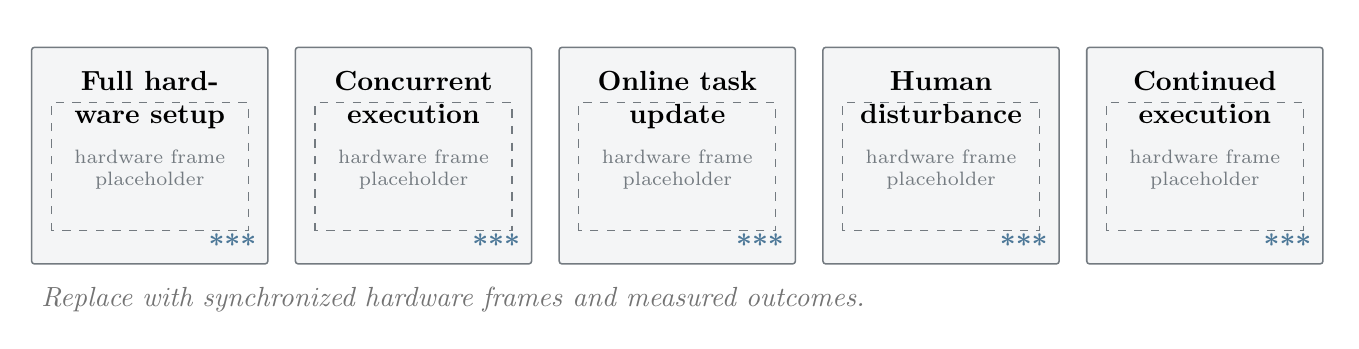
\begin{tikzpicture}[x=1cm,y=1cm,font=\rmfamily\fontsize{7.1}{7.9}\selectfont]
  \definecolor{hborder}{HTML}{737A80}
  \definecolor{hfill}{HTML}{F4F5F6}
  \definecolor{haccent}{HTML}{4D7898}
  \foreach \x/\title in {
    0/{Full hardware setup},
    3.35/{Concurrent execution},
    6.70/{Online task update},
    10.05/{Human disturbance},
    13.40/{Continued execution}
  }{
    \draw[hborder,fill=hfill,line width=0.55pt,rounded corners=1pt]
      (\x,0) rectangle (\x+3.0,2.75);
    \node[anchor=north,font=\bfseries,align=center,text width=2.7cm]
      at (\x+1.50,2.57) {\title};
    \draw[hborder,dashed,line width=0.45pt]
      (\x+0.25,0.42) rectangle (\x+2.75,2.05);
    \node[align=center,text=hborder] at (\x+1.50,1.20)
      {hardware frame\\placeholder};
    \node[text=haccent,font=\bfseries] at (\x+2.55,0.25) {***};
  }
  \node[anchor=west,text=black!55,font=\itshape] at (0,-0.45)
    {Replace with synchronized hardware frames and measured outcomes.};
  \path[use as bounding box] (-0.05,-0.65) rectangle (16.50,3.0);
\end{tikzpicture}
